\documentclass[a4paper, 12pt]{article}

\usepackage{amsmath}
\usepackage{graphicx}
\usepackage{caption}

\begin{document}

\title{Finite Impulse Respons system (FIR) - discrete convolution}
\date{}
\maketitle

\section{Introduction}

FIR systems are commonly used for digital signal processing. They can do signal filtration when used as filters or discrete convolution. These are the most popular applications of FIR systems. 

As name says FIR system has impulse response of finite durations. That means if we drive discrete delta impulse at FIR input its respons will setls down to zero in finite time. Discrete delta impuls can be written as:

\begin{align}
	\delta(n) = 
	\left\{
		\begin{array}{ll}
			1 & \mbox{if } x = 0 \\
			0 & \mbox{if } x \neq 0
		\end{array}
	\right.		
\end{align}

Mathematical record of finite respons on delta impulse should looks like:

\begin{align}
	g(n) =
	\left\{
		\begin{array}{ll}
			b_n & \mbox{if } 0 \leq n \leq M \\
			0, & \mbox{if } n > M		
		\end{array}
	\right.
\end{align} where b\textsubscript{n} represents impulse response in particular time step n, and M is response length. Output equation of FIR systems can be written as:

\begin{equation}\label{eq:FIR output equation}
y(n) = \sum_{i=0}^{n}{b_{i} \cdot u(n-i)}
\end{equation}

Having all that in mind one possible implementation of system with output equation like \eqref{eq:FIR output equation} is shown in figure \ref{fig:FIR block diagrame}.

\begin{figure}[h]
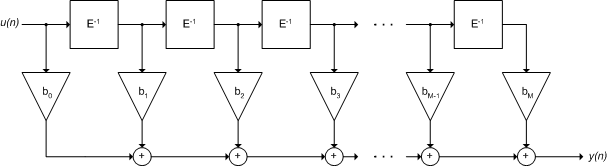
\includegraphics[width=1.0\textwidth=•]{/tools/home/pg_dsp/docs/images/FIR_block_diagrame.png}
\caption{FIR block diagrame}
\label{fig:FIR block diagrame}
\end{figure}

Translation of building block in figure \ref{fig:FIR block diagrame} to digital hardware is straightforward. Just replace adding block with adder, gain block with multiplier, and delay block (E\textsuperscript{-1}) with register. One possible implementation could be to copy block diagrame directly to some HDL code but that would not be general enough. We suggest another one shown in figure \ref{fig:Sequential FIR calculation}. As we can see, there is a memory storage for coefficients, and multiply accumulate unit that do summation from equation \ref{eq:FIR output equation}. Inputs named coefficients are loaded before computation. After loading surrounding hardware should start streaming data samples through samples interface. Connection from samples bus to coef memory is here just to indicate that we need mechanism to synchronize input samples with appropriate coefficient from memory. Later we will show how to do that efficiently using PyGears.

\begin{figure}[h]
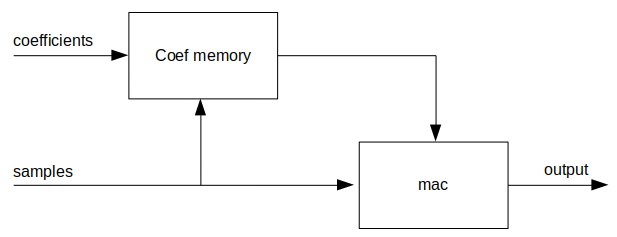
\includegraphics[width=1.0\textwidth=•]{/tools/home/pg_dsp/docs/images/Sequential_FIR.png}
\caption{Sequential FIR implementation block diagrame}
\label{fig:Sequential FIR calculation}
\end{figure}


Let's go back to the figure \ref{fig:FIR block diagrame}. Beside it will be slow in terms of frequency because of long combinational path, it will not be optimal regarding silicon needed for implementation. It will use M+1 multipliers and M adders. Because of that, we implement hardware that calculate FIR output sequentially. First, delay registers were removed outside the hardware block assuming that some other component will drive input sequence correctly. That means that current input sample and delayed ones will be driven as stream. If we look at equation \eqref{eq:FIR output equation} this stream is represented by $u(n-i)$ part which sould be multiplied with appropriate coefficient b\textsubscript{i}. Because FIR coefficient will be used over and over again a decision is made to store coefficient in memory module inside the hardware. Another reason for such implementation is caused by idea to make hardware reusable for more general mathematical operation behind the equation \eqref{eq:FIR output equation} called convolution because order of samples could vary.

\section{Implementation}

\end{document}
